% !TEX encoding = UTF-8 Unicode
\documentclass{article}           % use "amsart" instead of "article" for AMSLaTeX format
\usepackage{geometry}                           % See geometry.pdf to learn the layout options. There are lots.
\geometry{letterpaper}                          % ... or a4paper or a5paper or ... 
%\geometry{landscape}                           % Activate for for rotated page geometry
%\usepackage[parfill]{parskip}                  % Activate to begin paragraphs with an empty line rather than an indent
\usepackage{graphicx}                           % Use pdf, png, jpg, or eps§ with pdflatex; use eps in DVI mode
                                                % TeX will automatically convert eps --> pdf in pdflatex                

\usepackage[utf8]{inputenc}
\usepackage[T1]{fontenc}

\usepackage{amssymb}
\usepackage{amsmath}
\usepackage{amsthm}

\usepackage{caption}
\usepackage{subcaption}

\usepackage{tikz}
\usetikzlibrary{arrows}
\usetikzlibrary{shapes, arrows.meta}

\usepackage{../tex/mathpartir}
\usepackage{url}

\newtheorem{definition}{Definition}
\newtheorem{lemma}{Lemma}
\newtheorem{theorem}{Theorem}
\newtheorem{corrolary}{Corrolary}
\newtheorem{claim}{Claim}
 
\newcommand{\R}{\mathbb{R}}
\newcommand{\lowerT}[1]{\overrightarrow{#1}}
\newcommand{\cov}{\vartriangleleft}
\newcommand{\Pos}{\mathsf{Pos}}
\newcommand{\List}[1]{\mathsf{List}\ {#1}}
\newcommand{\fun}[2]{\lambda {#1}.\  {#2}}
\newcommand{\nat}{\mathbb{N}}
\newcommand{\rat}{\mathbb{Q}}
\newcommand{\suchthat}{\ |\ }
\newcommand{\concat}{\ensuremath{+\!\!\!\!+\,}}
\newcommand{\One}{\mathsf{One}}
\newcommand{\Dist}[1]{\mathcal{M}({#1})}
\newcommand{\Open}[1]{\mathcal{O}({#1})}
\newcommand{\coinflip}{\mathsf{coinflip}}
\newcommand{\Sampler}{\mathsf{Sampler}}
\newcommand{\bool}{\mathbb{B}}
\newcommand{\cons}{::}
\newcommand{\un}[1]{\ \mathrm{#1}}
\newcommand{\irule}[1]{\textsc{#1}}
\newcommand{\Type}{\mathcal{U}}
\newcommand{\Prop}{\mathcal{P}}

\newcommand{\Space}{\mathsf{Space}}
\newcommand{\Prob}{\mathcal{P}}
\newcommand{\Viet}{{\mathcal{V}^+}}

\newcommand{\map}[1]{\mathsf{map}_{#1}}
\newcommand{\ret}[1]{\mathsf{ret}_{#1}}
\newcommand{\join}[1]{\mathsf{join}_{#1}}

\newcommand{\truncate}[1]{\mathsf{trunc}\left({#1}\right)}

\newcommand{\ve}[1]{\mathbf{#1}}

\newcommand{\then}{\ ;\ }

\newcommand{\defeq}{\triangleq}

\title{Applications of formal topology}
\author{Ben Sherman}
%\date{\today}                                  % Activate to display a given date or no date

\begin{document}
\maketitle

What are potential applications of my framework for formal topology?

\section{The powerspaces: reasoning with and simulating uncertainty}

Why do we need a new programming language where types are topological spaces and expressions are continuous maps? After all, if one programs in Martin-Löf type theory (without axioms), then, as Escardó says \cite{escardo4wft}, ``Secretly, types are \emph{spaces} and functions are \emph{continuous}.''

The issue is that this fact is a metatheorem, and so one cannot intrinsically reason about topology within Martin-Löf type theory. Or at the very least, the topology is necessarily very sensitive to which axioms are employed. In particular, the existence of type whose topology as a space is not discrete is incompatible with the law of the excluded middle (LEM). So if one really wishes to reason about this ``intrinsic'' topology in Martin-Löf type theory, one must necessarily employ anti-classical axioms (i.e., axioms which violate LEM). One such axiom is Brouwer's continuity principle, which says that all functions on the Baire space ($\nat \to \nat$) are (pointwise) continuous:\footnote{The $\exists$ quantifier must be interpreted as ``mere'' existence or truncated existence, or it is not consistent\cite{escardo2015inconsistency}.}
\[
\forall f : (\nat \to \nat) \to \nat, 
\forall \alpha : \nat \to \nat,
\exists n : \nat,
\forall \beta : \nat \to \nat,
\alpha =_n \beta
\to
f \alpha = f \beta,
\]
where $\alpha =_n \beta$ means that the sequences $\alpha$ and $\beta$ agree on the first $n$ values.

A similar axiom is the uniform continuity principle, which states that all functions on the Cantor space ($\nat \to \bool$) are uniformly continuous:
\[
\forall f : (\nat \to \bool) \to \bool,
\exists n : \nat,
\forall \alpha, \beta : \nat \to \bool,
\alpha =_n \beta
\to
f \alpha = f \beta.
\]

An issue with adding these axioms (other than violating LEM, which seems to make people uncomfortable) is that they don't have any computational interpretation, so it is impossible to program using them.

My goal, with my programming language for formal topology, is to create a world where types are spaces, and expressions are continuous maps, and it is no secret! Making the topological nature of the programming language overt\footnote{No pun intended.}, and computable, has several advantages. Not only does it provide an alternative way to think about writing programs, but it also opens up new computational and reasoning possibilities that are not available with Martin-Löf type theory with its ``intrinsic topology.''

This article explore how these newfound capabilities manifest with ``powerspaces'', topological spaces whose points are in some sense collections of points of another topological space. If we let $\Space$ denote the type of topological spaces, then the powerspaces have type $\Space \to \Space$. In particular, they are monads. It will focus on two specific powerspaces: the inhabited Vietoris powerspace $\Viet$, and the probabilistic powerspace $\Prob$.

With these powerspaces, it is possible to both \emph{compute} with and \emph{reason} about non-determinism. The inhabited Vietoris powerspace represents demonic and angelic nondeterminism, while the probabilistic powerspace represents probabilistic non-determinism. In particular, we can lift  computation $f : A_1 \times \cdots \times A_n \to B$ defined on points to the lifted computation $f_\Viet : \Viet(A_1) \times \cdots \times \Viet(A_n) \to \Viet(B)$ which tracks how angelic/demonic uncertainty in inputs affects the output, or similarly, a lifted computation $f_\Prob : \Prob(A_1) \times \cdots \times \Prob(A_n) \to \Prob(B)$ which tracks how (independent) probabilistic uncertainty in inputs results in a probabilistically uncertain output. The ability to define these lifted computations is a straightforward consequence of the monadicity of $\Viet$ and $\Prob$.

Let's be more concrete. We consider the following task from the Uncertain<T> paper \cite{uncertaint}. Somebody is walking with their mobile phone, which has a GPS device. Periodically, the phone polls the GPS and estimate's the user's walking speed. If we think that the user is walking faster than 4 mph, we'd like to sound an alarm to warn the user to slow down, but we'd prefer false negatives (the user is walking faster than 4mph but we don't catch it) to false positives (the user is walking slower than 4mph but we sound the alarm).

The naïve approach this program simply takes point estimates from the GPS and computes the speed with those coordinates, and checks whether it is larger than 4mph to determine whether to alarm the user. We can think of this computation as a function which takes the two position coordinates whose time difference is $\Delta t > 0$ as input and estimates the speed accordingly:
\begin{align*}
\mathsf{compute\_speed} : \R^2 \times \R^2 &\to \R
\\ \mathsf{compute\_speed} (x_1, y_1) (x_2, y_2) &= \frac{1}{\Delta t} \sqrt{(x_2 - x_1)^2 + (y_2 - y_1)^2}.
\end{align*}
As \cite{uncertaint} points out, this fails to account for the uncertainty in the GPS position estimates, an in particular we are likely to overestimate the user's speed with this strategy, and alarm the user much too frequently.

We can explicitly take into account possible errors in the GPS coordinates in two ways. The simpler one is to model the GPS with non-determinism. For instance, we imagine that there was a real position $\ve{x}$ obscured with some additive noise $\ve{n}$ such that the magnitude of the noise is not too large, i.e., $\| \ve{n} \| \le \varepsilon$ for some $\varepsilon \ge 0$.

By modeling such non-determinism with the Vietoris powerspace, we can automatically lift the $\mathsf{compute\_speed}$ map to one that operates on uncertain positions to produce an uncertain speed estimate. Then, instead of asking the question whether our speed estimate is greater than 4mph, we can ask: Is the speed \emph{necessarily} greater than 4mph? Is the speed \emph{possibly} greater than 4mph? We can \emph{compute} the answer to these questions, in a strong sense, as we could compute whether a single speed estimate is greater than 4mph.

Another way to take into account the uncertainty of the GPS estimates, which is probably more appropriate in this case, is to model the GPS estimates as corrupted with a probabilistic noise. So our real position $\ve{x}$ is obscured with additive noise $\ve{n}$ which is drawn from a normal distribution with mean 0 and variance $\sigma^2$. Now, for each real number $p : \R$ such that $0 \le p < 1$, we can ask whether the probability that the speed is greater than 4mph is greater than $p$, and again, this is computable in the same sense as the previous analogous questions.

The remainder of this article will give a vague and incomplete explanation of how formal topology works, how the powerspaces are defined, and how we can solve the above task with formal topology.

In the constructive formulation of topological spaces, spaces are just logical theories in a restricted fragment of logic known as \emph{propositional geometric logic}. In this fragment of logic, we are only allowed to use finite conjunctions and infinitary disjunctions; no implication or negation. The formulae in these theories represent \emph{observable} properties of a space. They are also called \emph{opens}, because they represent what would be the open sets in conventional topology. For instance, the real numbers $\R : \Space$ are defined by the theory with atomic propositions $a < \cdot < b$ for each $a, b : \rat$ such that $a < b$, which are just syntactic objects which represent the proposition that a real number is greater than $a$ and less than $b$. The theory then has the following axioms which relate the propositions:

\begin{figure}[h!]
\caption{Logic of observables for $\R$.}
\label{Rcov}
\begin{center}
\begin{subfigure}[t]{0.4\textwidth}
\begin{center}
 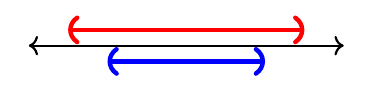
\begin{tikzpicture}
 \draw [<->, thick] (-2, 0) -- (2, 0);
 \draw [(-), ultra thick, blue] (-1, -0.2) -- (1, -0.2);
 \draw [(-), ultra thick, red] (-1.5, 0.2) -- (1.5, 0.2);
 \end{tikzpicture}
 \end{center}
\begin{mathpar}
\inferrule* [right=widen]
  {p' \le p < q \le q' }
  {p < \cdot < q \vdash p' < \cdot < q'}
\end{mathpar}
\end{subfigure}
~
\begin{subfigure}[t]{0.4\textwidth}
\begin{center}
 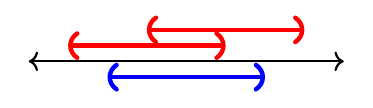
\begin{tikzpicture}
 \draw [<->, thick] (-2, 0) -- (2, 0);
 \draw [(-), ultra thick, blue] (-1, -0.2) -- (1, -0.2);
 \draw [(-), ultra thick, red] (-1.5, 0.2) -- (0.5, 0.2);
  \draw [(-), ultra thick, red] (-0.5, 0.4) -- (1.5, 0.4);
 \end{tikzpicture}
 \end{center}
\begin{mathpar}
\inferrule* [right=split]
  {r < p < u < s < q < v}
  {p < \cdot < q \vdash r < \cdot < s \ \vee\  u < \cdot < v }
\end{mathpar}
\end{subfigure}

\vspace{1em}

\begin{subfigure}[t]{0.4\textwidth}
\begin{center}
 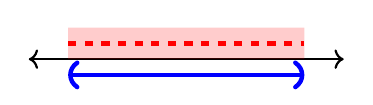
\begin{tikzpicture}
 \draw [<->, thick] (-2, 0) -- (2, 0);
 \draw [(-), ultra thick, blue] (-1.5, -0.2) -- (1.5, -0.2);
 \draw [ultra thick, dashed, red] (-1.5, 0.2) -- (1.5, 0.2);
  \fill[fill=red, opacity=0.2]  (-1.5, 0)--(-1.5,0.4)--(1.5,0.4)--(1.5,0)--(-1.5,0);
 \end{tikzpicture}
 \end{center}
\begin{mathpar}
\inferrule* [right=inside]
  { }
  {p < \cdot < q \vdash \bigvee \{ x < \cdot < y \suchthat p < x < y < q \}}
\end{mathpar}
\end{subfigure}

\end{center}
\end{figure}

The opens are observable, in the sense that if it is a theorem for a space that some (possibly infinitary) disjunction holds, i.e.,
\[
\top \vdash \bigvee_{i : I} P(i),
\]
then a point of a space can \emph{compute} some proposition of that disjunction which holds of that particular point. Said in a more spatial language, the above theorem represents an open cover of a space, and a point can \emph{compute} for any such open cover an open set of that cover which it lies in. A point is defined by the observable propositions that hold of it, i.e., the opens that it lies in. For a point $x : \R$ and open $P : \Open{\R}$, we write $x \models P$ (read ``$x$ lies in $P$'') if the property $P$ holds of $x$. Then we formally state the previously mentioned computation rule for points as \footnote{We assume that we are working in a constructive metatheory, and read the existential in the conclusion of \irule{split-cov} as constructive. That is, from the data in the hypothesis, one can compute the index $i : I$ of the disjunct which holds.}
\begin{mathpar}
\inferrule* [right=split-cov]
  {x \models P \qquad P \vdash \bigvee_{i : I} Q(i)}
  {\exists i : I, x \models Q(i) }
\end{mathpar}

We write $\Open{\R}$ to represent the opens of $\R$, so for any $a, b : \rat$ we have $a < \cdot < b : \Open{\R}$. It turns out that we can represent opens also as continuous maps from the space of interest to the Sierpínski space $\Sigma$, and it's convenient to conflate the two. For instance, for each open $a < \cdot < b : \Open{\R}$ we have a map
\[
\fun{x}{a < x < b} : \R \to \Sigma.
\]

Particularly, thinking in this way provides nice notation. For maps to the Sierpínski space, we may existentially quantify over certain spaces\footnote{overt spaces} such as $\rat \times \rat$, so we can for instance define for any $x : \R$ \footnote{I should probably explain what $b < q : \Sigma$ means and why it's okay to write.}
\[
x < q \defeq \exists (a, b) : \rat \times \rat, b < q \wedge a < x < b
\]
and building on this, we can for instance write for points $x, y : \R$,
\[
x < y \defeq \exists q : \rat, x < q \wedge q < y.
\]

So how can we write the naïve speed estimation program using formal topology? It should come as no surprise that operations such as addition, subtraction, multiplication, and square root can be defined, and so the $\mathsf{compute\_speed}$ function described above can be implemented exactly as written.

\subsubsection{Making Boolean decisions on connected spaces}
But in the floating-point version of naïve speed estimation program, we can then simply check whether the estimated speed exceeds 4, and decide whether to sound the alarm based on that boolean check. This is not possible for $\R$, and I'd argue that the discrepancy should be viewed as a deficiency in floating point rather than of $\R$. The ordering of two real numbers is undecidable; our estimated speed could be arbitrarily close to 4, and we wouldn't know whether it is exactly 4 or whether it exceeds 4. The topological explanation of this is that $\R$ is connected, and so there is no non-constant continuous map from $\R$ to $\bool$.

The more appropriate way to make decisions from $\R$ is to provide an open cover of $\R$, together with an acceptable computation for each open in the open cover. I like to think of this as an overlapping pattern match. In general, we need two local computations to ``agree'' whenever their corresponding opens overlap for a suitable definition of agreement.

There is a convenient topological space which describes Boolean decisions where it is sometimes acceptable to make either decision. We'll call the space $\mathsf{Decision} : \Space$.
\footnote{I could also imagine a general construction of spaces $X \oplus Y$ called a ``fuzzy union'', where $\mathsf{Decision} = \mathsf{unit} \oplus \mathsf{unit}$, and this would be the best space for the car being before or after the intersection.}
 It has two basic propositions $\mathsf{L}$ and $\mathsf{R}$, which can be read as indicating that it is acceptable to make the ``left'' or the ``right'' decision, respectively. And it has a single axiom,
\[
\top \vdash \mathsf{L} \vee \mathsf{R},
\]
which says that it must always be acceptable to make one of the choices. It turns out that $\mathsf{Decision}$ has three points, which have the following observable properties:
\begin{align*}
\mathsf{only\_L} &\models \mathsf{L}
& \mathsf{only\_R} & \nvDash \mathsf{L}
& \mathsf{both} &\models \mathsf{L}
\\
\mathsf{only\_L} &\nvDash \mathsf{R}
& \mathsf{only\_R} & \models \mathsf{R}
& \mathsf{both} &\models \mathsf{R}.
\end{align*}

It is useful to consider the \emph{specialization preorder} $\le$, which is a preorder on the points of any space. We have for any points $x, y : A$
\[
x \le y \defeq \forall P : \Open{A}, x \models P \to y \models P,
\]
which means that any property which holds of $x$ must also hold of $y$. For many conventional topological spaces, such as $\R$, the specialization order is discrete, but $\mathsf{Decision}$ has an interesting specialization preorder, as we can draw the Hasse diagram below:
\begin{center}
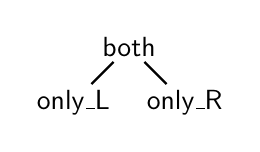
\begin{tikzpicture}
    \node (top) at (0,0) {$\mathsf{both}$};
    \node [below left  of=top] (left)  {$\mathsf{only\_L}$};
    \node [below right of=top] (right) {$\mathsf{only\_R}$};

    % Now draw the lines:
    \draw [thick, shorten <=-2pt, shorten >=-2pt] (top) -- (left);
    \draw [thick, shorten <=-2pt, shorten >=-2pt] (top) -- (right);
\end{tikzpicture}
\end{center}

We can think of opens (in this case $\mathsf{L}$ and $\mathsf{R}$) as behaviors as well, in which case $x \le y$ means that $y$ can always ``choose'' to behave as $x$, in the sense that $y$ could potentially be indistinguishable from $x$. So the Hasse diagram tells us that $\mathsf{both}$ might choose to behave as $\mathsf{only\_L}$ or it may choose to behave as $\mathsf{only\_R}$.

There is a convenient map
\begin{align*}
\mathsf{decide} : \{ (\ell, r) : \Sigma \times \Sigma \suchthat \ell \vee_\Sigma r \} \to \mathsf{Decision}
\\ \mathsf{decide}(\ell, r) = \mathsf{cases}(\ell, r)
\begin{cases}
\fun{(\ell, r)}{\ell}
  \quad &\Longrightarrow \quad \mathsf{only\_L}
\\
\fun{(\ell, r)}{r}
  \quad &\Longrightarrow \quad \mathsf{only\_R}
\end{cases}
\end{align*}

which converts two possible observations $\ell$ and $r$, where we know that one or the other must hold, into a $\mathsf{Decision}$. Upon giving the above definition, we are faced with two proof goals to confirm that the definition is well-formed. First, we must prove
\[
\checkmark(\ell \vee_\Sigma r) \vdash \checkmark(\ell) \vee \checkmark(r),
\]
for $\ell, r : \Sigma$ to show that the $\mathsf{cases}$ construct covers all possible cases, which is trivial since
\[
\checkmark(\ell \vee_\Sigma r) = \checkmark(\ell) \vee \checkmark(r)
\]
by the definition of $\vee_\Sigma$. We must then prove that overlapping cases can be reconciled. For this definition, the proof goal is effectively to find a point which is the ``maximum'' of $\mathsf{only\_L}$ and $\mathsf{only\_R}$ with respect to the specialization preorder; $\mathsf{both}$ suffices as such a maximum.

In fact, the two spaces in the type signature of $\mathsf{decide}$ are homeomorphic, with $\mathsf{decide}$ giving one part of that homeomorphism.

[[ How to get answers out of a decision? Probe it with the one axiom of the theory]]

So our decision procedure to sound the alarm might look like this:
\begin{align*}
\mathsf{sound\_alarm?} : \R &\to \mathsf{Decision}
\\ \mathsf{sound\_alarm?}(x) &= \mathsf{decide}(x > 4.0, x < 4.1)
\end{align*}

To complete writing this program, we will be presented with a (geometric) proof obligation
\[
x > 4.1 \vee x < 4.0
\]
in the context $x : \R$. What happens when a point satisfies multiple possible cases? Then the decision that is made will depend upon the point's computational behavior. Recall that in the \irule{split-cov} rule, a point much choose an open from an open cover which it lies in. If a point lies in more than 1 of those opens, it may choose any of them, and therefore different implementations of the same point may make different computational choices. So depending on the implementation of a point for the real number 4.05, the alarm may or may not sound.

So this represents what the naïve computation might look like in formal topology. Now, let's define the inhabited Vietoris powerspace, and extend the speed estimation example to this sort of non-determinism.

The inhabited Vietoris powerspace $\Viet$ represents non-determinism. For a space $A$, the points of a $\Viet(A)$ are certain ``tractable'' nonempty subspaces of $A$. We will call these subspaces which are points of $\Viet(A)$ \emph{compact/overt}. If a space $A : \Space$ has an open $P : \Open{A}$, then the Vietoris powerspace has opens $\square P : \Open{\Viet(A)}$ as well as $\lozenge P : \Open{\Viet(A)}$. \footnote{Notation is borrowed from modal logic.} Viewing $P$ as a proposition that may hold of points of $A$, $\square P$ indicates whether $P$ \emph{necessarily} holds everywhere in the subspace, while $\lozenge P$ indicates whether $P$ \emph{possibly} holds somewhere in the subspace. Therefore, for a point $s : \Viet(A)$, we'll use the following notation for the $\Sigma$-valued continuous maps:
\begin{align*}
\forall x \in s, e &\defeq s \models \square (\fun{x}{e})
\\ \exists x \in s, e &\defeq s \models \lozenge (\fun{x}{e}),
\end{align*}
where the expression $e$ has $x$ as a free variable. 

[[Remove this?:]] The above notation isn't formally meaningful, so perhaps it's better demonstrated with an example:
\[
\forall x \in s, x < a \vee x > b
\quad \defeq \quad 
s \models \square 
  \left(\bigvee \{ (p, q) : \rat \times \rat
     \suchthat q < a \vee p > b \} \right)
\]

[ Should give more explanation, should say how these are relatively strong computational properties ]

There is a theorem, which we will call Heine-Borel, as it is analogous to similar theorems of that name, which says that any closed interval of $\R$ is compact/overt. More formally, there is a map
\[
f : \{ (a, b) : \R \times \R \suchthat a < b \} \to \Viet(\R)
\]
such that for every $(a, b) : \R \times \R$ such that $a < b$, we have
\begin{align*}
\forall x \in f(a, b), p < x < q \qquad &\defeq \qquad a < p \wedge q < b
\\ \exists x \in f(a, b), p < x < q \qquad &\defeq \qquad p < b \vee a < q.
\end{align*}

The Heine-Borel theorem has an adjoint: any compact set in $\R$ has a minimum and maximum. So we can define the continuous map $\max : \Viet(\R) \to \R$ as follows:
\begin{align*}
p < \max(s) < q
\qquad \defeq \qquad 
\left( \exists x \in s, p < x \right) \wedge \left( \forall x \in s, x < q \right).
\end{align*}

The Vietoris powerspace is functorial, i.e., applying any continuous map $f : A \to B$ ``pointwise'' to a compact/overt set yields another compact/overt set, so there is a continuous map $\map{\Viet}{f} : \Viet(A) \to \Viet(B)$. The specification of this map is unsurprising:
\begin{align*}
\forall y \in \map{\Viet}{f}(s), P(y) \qquad &\defeq \qquad \forall x \in s, P(f(x))
\\ \exists y \in \map{\Viet}{f}(s), P(y)  \qquad &\defeq \qquad \exists x \in s, P(f(x)).
\end{align*}

Furthermore, the Vietoris powerspace is monadic. For any point $x : A$ there is the compact/overt set $\ret{\Viet}(x) : \Viet(A) $ consisting of that single point:
\begin{align*}
\forall y \in \ret{\Viet}(x), P(y) \qquad &\defeq \qquad P(x)
\\ \exists y \in \ret{\Viet}(x), P(y) \qquad &\defeq \qquad P(x).
\end{align*}
And we can collapse nested nondeterminism in the way we'd expect as well, with $\join{\Viet} : \Viet(\Viet(A)) \to \Viet(A)$:
\begin{align*}
\forall x \in \join{\Viet}(s), P(x) \qquad &\defeq \qquad \forall s' \in s, \forall x \in s', P(x)
\\ \exists x \in \join{\Viet}(s), P(x) \qquad &\defeq \qquad \exists s' \in s, \exists x \in s', P(x).
\end{align*}

Let's use the Vietoris powerspace to enable us to compute with uncertain values of our GPS estimates. Recall that we're imagining that the true position $\ve{x}$ is corrupted by some noise $\ve{n}$ that lies in a closed circular disk, i.e., $\| \ve{n} \| \le \varepsilon$ for some $\varepsilon \ge 0$. For simplicity, assume $\varepsilon = 1$. Then our noise is the unit disk in $\R^2$. We should be able to represent this as a point of $\Viet(\R)$ because it is a compact/overt subspace of $\R^2$. We can explain this in two steps. First, the square 
\[
\{ (x, y) : \R \suchthat -1 \le x \le 1 \wedge -1 \le y \le 1 \}
\]
is compact/overt because it is the product of two intervals, which are each compact/overt by the Heine-Borel theorem. The fact that the product of two compact/overt subspaces is compact is known as the binary Tychonoff theorem, $\otimes : \Viet(A) \times \Viet(B) \to \Viet(A \times B)$. Noting that the basic opens of a product space are the product of the basic opens, the specification should look something like this:\footnote{This is super sloppy and even though it might intuitively get the idea across, it's probably wrong. The issue (throughout this whole explication) is whether the basis for the Vietoris space is essentially the same size as the basis for the original space. I would need to think about it.}
\begin{align*}
s \otimes t &\models \square (P, Q) \qquad \text{iff} \qquad s \models \square P \wedge t \models \square Q
\\ s \otimes t &\models \lozenge (P, Q) \qquad \text{iff} \qquad s \models \lozenge P \wedge t \models \lozenge Q.
\end{align*}

Next, we know that the unit disk is closed, since it is co-classified by the open set
\[
\fun{(x,y)}{x^2 + y^2 > 1}.
\]
The intersection of a compact/overt space with a closed overt space is still compact/overt\footnote{I need to go back and do this better. I should describe the lower and upper powerspace, so that the closed space being overt is being a point of the upper powerspace}. Given a compact/overt set $s : \Viet{A}$ and an open $U : \Open{A}$ co-classifying a desired closed set, the intersection $s \cap U^c$ is specified by
\begin{align*}
s \cap U^c &\models \square P \qquad \text{iff} \qquad s \models \square (P \vee U)
\\ s \cap U^c &\models \lozenge P \qquad \text{iff} \qquad [[\text{BROKEN}]].
\end{align*}

With this, we can imagine that we have the desired term $\mathsf{unit\_disk} : \Viet(\R^2)$. Then our speed estimation program which takes into account the uncertainty can be written like this, using ``syntactic sugar'' for monadic operations:
\begin{align*}
\mathsf{compute\_speed}_\Viet : \R^2 \times \R^2 &\to \Viet(\R)
\\ \mathsf{compute\_speed}_\Viet (\ve{x}_1, \ve{x}_2) &= 
  \ve{n}_1 \leftarrow \mathsf{unit\_disk} 
  \then
  \ve{n}_2 \leftarrow \mathsf{unit\_disk}
  \then
  \\ &\ret{\Viet} \left( \mathsf{compute\_speed}(\ve{x}_1 - \varepsilon \ve{n}_1, \ve{x}_2 - \varepsilon \ve{n}_2) \right).
\end{align*}

Note that I subtract the noise rather than add it. Of course, due to symmetries of the unit disk, it doesn't matter here. But there's a small subtlety in the more general case: we imagined that the \emph{real} position was corrupted with some noise which was added to it. But we have the \emph{noisy} position, and want to find all the possible real positions which could yield this noisy one. With any additive noise, we can do this simply via subtraction. However, with a more general noise kernel, this inversion process isn't necessarily so easy.

What do we do now that we have a speed estimate, $s : \Viet(\R)$, which comes with uncertainty, when it comes to deciding whether to sound the alarm. If we use this program
\begin{align*}
\mathsf{sound\_alarm?}_\Viet : \Viet(\R) &\to \mathsf{Decision}
\\ \mathsf{sound\_alarm?}_\Viet(s) &= \mathsf{decide}((\forall x \in s, x > 4.0) , (\exists x \in s, x < 4.1))
\end{align*}
we will be conservative in accordance with our uncertainty; we only sound the alarm if \emph{necessarily} the user's speed is greater than 4mph. Writing this program gives us the proof obligation
\[
\left( \forall x \in s, x > 4.0 \right) \vee \left( \exists x \in s, x < 4.1 \right)
\]
in the context $s : \Viet(\R)$, and intuitively we see that it must hold. Another way to see this is to note the equivalence 
\[
\mathsf{sound\_alarm?}_\Viet(s) = \mathsf{sound\_alarm?}(\max(s)).
\]

The whole program is 
\[
\mathsf{sound\_alarm?}_\Viet \circ \mathsf{compute\_speed}_\Viet : \R^2 \times \R^2 \to \mathsf{Decision}.
\]
Note that the $\Viet$ doesn't occur in the types, as it was only used in intermediate computations. Using $\Viet$ allowed us to conveniently write a program that deals with the uncertainty inherent in GPS coordinates. While it is convenient, it is not necessarily efficient, and in the special case where we have additive noise from the unit disk, we can just do a worst-case speed estimate
\begin{align*}
\mathsf{compute\_max\_speed} &: \{ (\ve{x}_1, \ve{x}_2) : \R^2 \times \R^2 \suchthat \ve{x}_1 \ne \ve{x}_2 \} \to \R
\\ \mathsf{compute\_max\_speed} (\ve{x}_1, \ve{x}_2) &= 
\mathsf{let}\ \ve{d} = \ve{x}_2 - \ve{x}_1\ \mathsf{in}\ 
\\
&\mathsf{compute\_speed}\left( 
\ve{x}_1 - \varepsilon \frac{\ve{d}}{\| \ve{d} \|}, \ve{x}_2 + \varepsilon \frac{\ve{d}}{\| \ve{d} \|}
\right).
\end{align*}
The above program is not defined when $\ve{x}_1 = \ve{x}_2$, but since it is defined on a dense subspace of $\R^2 \times \R^2$, it admits a (unique) continuous extension to the entire space (in this case, the speed estimate when $\ve{x}_1 = \ve{x}_2$ will be $\frac{2\varepsilon}{\Delta t}$).
Once we've extended the above program, we should be able to prove (with much effort) the equivalence of the programs
\[
\mathsf{sound\_alarm?}_\Viet \circ \mathsf{compute\_speed}_\Viet
=
\mathsf{sound\_alarm?} \circ \mathsf{compute\_max\_speed}.
\]

In this case, we can think of the program which explicitly uses the inhabited Vietoris hyperspace as an executable specification, helping understand when we have found a more efficient program which accomplishes the same task. In particular, the program using $\Viet$ at the very least confirms that it is possible in principle to create such a program.

How does this beat existing approaches?

Suppose we simply wanted to program using MLTT, perhaps using data structures for the real numbers from the c-CoRN library. Then one cannot define meaningfully, for instance, the inhabited Vietoris powerspace for $\R$, as notions of continuity and compactness do not interact well, unless one accepts additional axioms. In particular, \cite{waaldijk} proves the following theorem:
\begin{quote}
Within \textsc{bish} the following statements are equivalent:
\begin{enumerate}
\item The fan theorem \textbf{FT}.
\item There exists a class of real-valued functions called `kontinuous' functions such that:
\begin{enumerate}
\item if $f$ is a uniformly continuous real-valued function defined on $[0, 1]$, then $f$ is kontinuous;
\item if $f$ and $g$ are kontinuous functions such that $\text{Ran}(f) \subseteq \text{Dom}(g)$, then the composition $g \circ f$ is kontinuous;
\item if $f$ is a kontinuous function defined on $[0, 1]$, then $f$ is
uniformly continuous;
\item the function $x \mapsto 1/x$, defined on $\R^+$, is kontinuous.
\end{enumerate}
\end{enumerate}
\end{quote}

Therefore, even \emph{reasoning} about such ideas is difficult in MLTT, and certainly there is no in-built mechanism for \emph{computing} in this manner. Whilst there may be ways around these difficulties, at the very least the concepts are not natural. So in MLTT, the best one could do is reason about nondeterminism using definitions as subsets of points; computing over those subsets is not possible.

Most of the concepts described thus far are also described in a similar way in Paul Taylor's Abstract Stone Duality (ASD). However, as far as I am aware, there is no notion of the $\mathsf{cases}$ construct in ASD, which is needed to make discrete decisions over connected spaces. The Marshall programming language is capable of doing some of the interesting computation described here, such as universal quantification over the unit disk\footnote{I'm still unsure about existential quantification over the unit disk, in general.}. However, since its only base type is $\R$, it does not have, for instance, the Vietoris powerspace as a first-class object.

[What other alternative approaches are there that I should claim are not as good as this approach?]

[Next, I should do the same rigmarole with the probabilistic powerspace.]

\section{How much do I need to sample?}

Mike asks, ``Perhaps the task at hand is to identify a space that enables us to ask
some of the following questions: Can we verify/minimize the number of sensor samples needed to verify a property with a given probability?''

Let's take a concrete example. Mike has a coin which he says is fair, but I don't trust him. He'll flip the coin for me for as long as I wish; I want to write a program which will call him out for his unfair coin once I'm certain that the coin is unfair with probability greater than 90\%. However, if I end up finding that the coin's bias seems to be between 45\% and 55\% with probability greater than 5\%, I'll say that I trust Mike and call it a day. And I'd like my response to be correct with greater than 95\% probability.

Let $\mathbb{I}$ represent the real numbers between 0 and 1 (inclusive). This is the parameter space for the problem, indicating the probability that the coin lands on heads. The sampling space for the coinflips is $\bool$, where we interpret $\mathsf{true}$ as heads and $\mathsf{false}$ as tails.

Let $p : \mathbb{I}$ represent the actual bias of Mike's coin. At first glance, my program looks trivial:
\begin{align*}
\mathsf{Mike\_honest?} &: \| \bool\|
\\ \mathsf{Mike\_honest?} &= \mathsf{cases}
\begin{cases}
\text{Pr}_{x \leftarrow \ret{\Prob}(p)} \left[ x \ne 0.5 \right] > 0.9
  \quad &\Longrightarrow
   \mathsf{trunc}(\mathsf{false})
\\
\text{Pr}_{x \leftarrow \ret{\Prob}(p)} \left[ 0.45 < x < 0.55 \right] > 0.05
  \quad &\Longrightarrow
   \mathsf{trunc}(\mathsf{true}).
\end{cases}
\end{align*}

But of course, I can't actually do this, because I don't have access to $p$. If I \emph{did} have access to $p$, there'd be no need for anything probabilistic; I could have just done
\begin{align*}
\mathsf{Mike\_honest?}_2 &: \| \bool\|
\\ \mathsf{Mike\_honest?}_2 &= \mathsf{cases}
\begin{cases}
p \ne 0.5 
  \quad &\Longrightarrow
   \mathsf{trunc}(\mathsf{false})
\\
0.45 < p < 0.55
  \quad &\Longrightarrow
   \mathsf{trunc}(\mathsf{true}).
\end{cases}
\end{align*}

Though we don't have access to $p$. Rather, we have access to a stream of coinflips $s : \mathsf{Stream}(A)$ drawn from $\prod^\omega \mathsf{bernoulli}(p)$. Additionally, we begin with a prior distribution $\mathsf{prior} : \Prob(\mathbb{I})$ on the bias of Mike's coin as well as an updating function $\mathsf{posterior} : \Prob(\mathbb{I}) \times \bool \to \Prob(\mathbb{I})$ which updates any prior with a new sample drawn from the distribution which we wish to do inference over. Thus, we get a sequence of posterior distributions as we take into account each new coinflip:
\begin{align*}
\mathsf{posteriors} &: \nat \to \Prob(\mathbb{I})
\\ \mathsf{posteriors}(0) &= \mathsf{prior}
\\ \mathsf{posteriors}(S(n)) &= \mathsf{posterior}(\mathsf{posteriors}(n), s[n]).
\end{align*}

I interpret that we have the following situation. We 

\section{Other applications}

\subsection{Everything dReal does}
Shows how simple the principles behind dReal are. Shows how easy it is to "program" dReal in formal topology. 

\subsection{Computing probabilities/sampling}
\subsection{Maximizing/minimizing functions over compact sets}
\subsection{Understanding decision-making in the continuous world}
\subsection{CAD}
\subsection{Robots}
\subsection{Similar things to what relaxed programs do in terms of ``approximate'' things}


\bibliographystyle{alpha}
\bibliography{Applications}

\end{document}
